\documentclass[12pt, a4paper]{article}
\setlength{\textheight}{24cm}
\setlength{\textwidth}{16cm}
\setlength{\topmargin}{0cm}
\setlength{\evensidemargin}{0cm}
\setlength{\oddsidemargin}{0cm}
\usepackage[affil-it]{authblk}
\usepackage{graphics}
\usepackage{graphicx}
\usepackage{caption}
\usepackage{float}
\begin{document}
\title{Comparison of some FFT libraries in C}
\author{Philippe Gambron \thanks{\texttt{philippe.gambron{@}stfc.ac.uk}}}
\affil{Science and Technology Facilities Council, Rutherford Appleton Laboratory, Hartree Centre, Harwell Campus, Harwell Oxford, OX11 0QZ, United Kingdom}
\maketitle
\begin{abstract}
We compare the performance, on a single node, of several libraries computing FFTs that can be called form C code. 
\end{abstract}
\section{Introduction}
\section{Overview of the chosen libraries}

We consider the libraries FFTW \cite{fftw}, MKL, GSL \cite{gsl} and FFTPACK \cite{fftpack} (Table \ref{ffttable}). They can perform complex transforms, real to half-complex (and conversely) and, in the case of, FFTW, real to real when the signal is odd or even. The half-complex output consists in half as many complex values as there were points in the signal, taking advantage of the hermiticity of the Fourier transform of a real function.\\

FFTW and MKL can compute FFTs in several dimensions and can work in a distributed way, using multihtreading and MPI. The purpose of this work is to asses their performance on a single node. As a consequence, we will only study the effect of multihtreading. 
\begin{table}[H]
\captionsetup{width=1\textwidth}
\begin{tabular}{|p{2.5cm}||p{2.5cm}|p{1cm}|p{3cm}|p{3cm}|p{2cm}|p{2cm}|}
\hline
& Type & Dim. & Radices & Parallelism & Licence \\
\hline
\hline
FFTW & R$\to$H,\ \ \  C$\to$C,\ \ \  H$\to$R, R{\scriptsize (odd/even)}$\to$R& Any&2, 3, 5, 7, 11, 13 + any with code generator & Multithreading, MPI & GPL v2\\
\hline
MKL  &  R$\to$H,\ \ \  C$\to$C,\ \ \ \  H$\to$C& Any & & Multithreading, MPI & Proprietary\\
\hline
GSL  &  R$\to$H,\ \ \  C$\to$C,\ \ \ \  H$\to$R & 1 & 2, 3, 5, 6, 7 & - & GPL v3\\
\hline
FFTPACK {\scriptsize (CASA wrapper)} &  R$\to$H,\ \ \  C$\to$C,\ \ \ \  H$\to$R & 1 & & - & GPL v2\\
\hline
\end{tabular}
\caption{Overview of the FFT libraries considered. R stands for real, C, for complex, and HC, for half-complex.}
\label{ffttable}
\end{table}
\section{Performance}

The performance measured for the transform, using FFTW and MKL, with a single thread, of a cube of complex values appears in Fig. \ref{perf3d}. Carrying out the transform in a single dimension allows us to benchmark GSL and FFTPACK\footnote{We have used the C++ wrapper of FFTPACK provided by CASA, the radioastronomy package \cite{casa} since FFTPACK is written in FORTRAN. Using the CASA header files and linking to its libraries is not supported. As a consequence, this was quite difficult to set up on Archer and required to use the libraries provided by an old version of Debian, to match the libraries available on the system.} as well as is illustrated in Fig. \ref{perf1d}.\\

According to our measurements, MKL performs the most efficiently. We have taken measurements for cube sides that are a power of 2, a product of small integers and primes. As expected, the performance is worse with primes than with powers of 2 or products of small integers. We also notice that the performance with primes is significantly worse in the cases of GSL and FFTPACK. We have observed that the flatness of the domain does not affect significantly the performance. For example, a flattened or elongated cuboid will yield a performance close to a cube containing the same number of elements.\\

Finally, we assess how the performance scales with an increasing number of threads. In this case, FFTW scales better but starts from a lower performance (Fig. \ref{perfmt}).
\begin{figure}[H]
\captionsetup{width=0.6\textwidth}
\centering
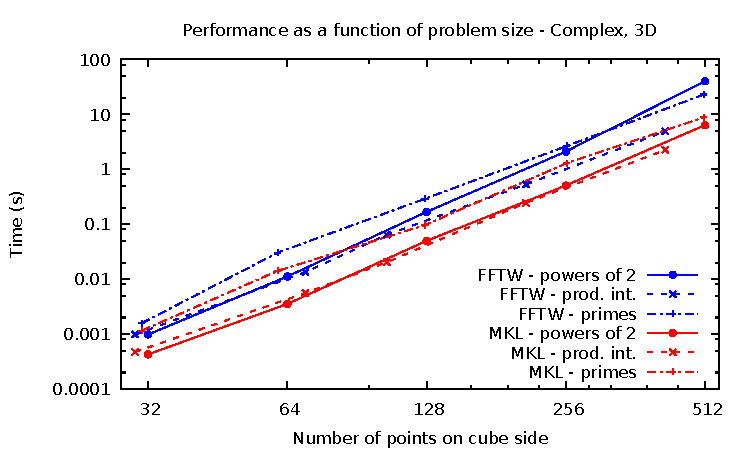
\includegraphics[height=8cm]{graphs/performance3dc/performance3dc.pdf}
\caption{Execution time as a function of the side of a cube of complex values (1 thread). The side of the cube can be a power of 2, a product of small integers or a prime number.}
\label{perf3d}
\end{figure}

\begin{figure}[H]
\captionsetup{width=0.6\textwidth}
\centering
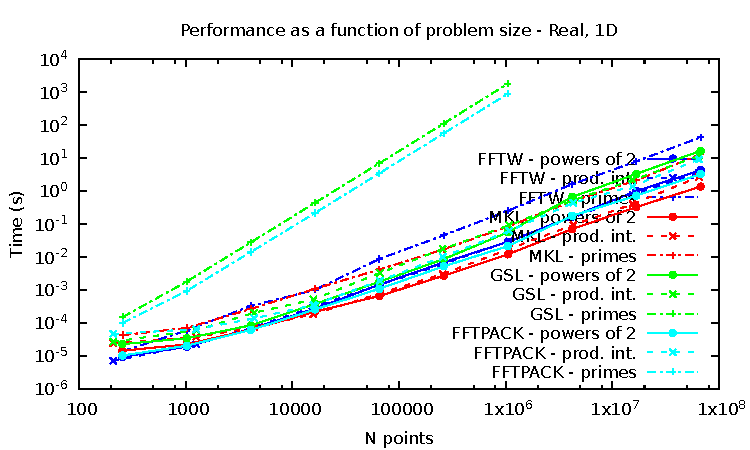
\includegraphics[height=8cm]{graphs/performance1dr/performance1dr.pdf}
\caption{Execution time as a function of the number of points, in one dimension and with real values (1 thread). The number of points can be a power of 2, a product of small integers or a prime number.}
\label{perf1d}
\end{figure}

\begin{figure}[H]
\captionsetup{width=0.6\textwidth}
\centering
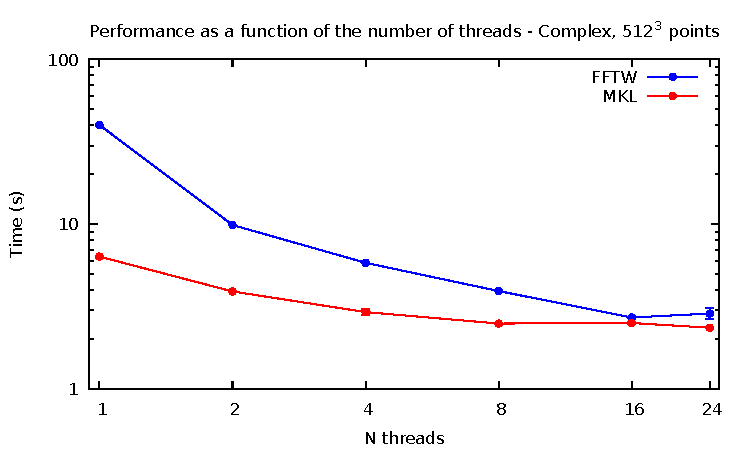
\includegraphics[height=8cm]{graphs/multithreading/multithreading.pdf}
\caption{Effect of the multithreading of the performance for a cube of $512^3$ complex values.}
\label{perfmt}
\end{figure}  

\begin{figure}[H]
\captionsetup{width=0.6\textwidth}
\centering
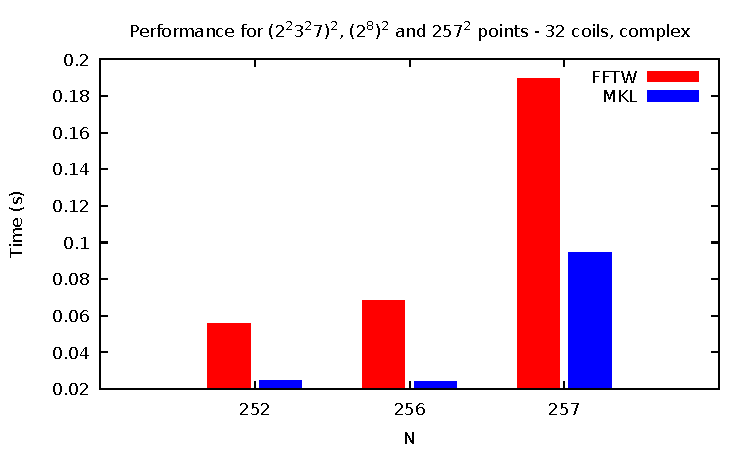
\includegraphics[height=8cm]{graphs/ccp/ccp.pdf}
\caption{The boundary conditions for several time steps are interpolated from the values on a coarse grid in space and time.}
\label{method}
\end{figure}

\section{Requirements from the CCP}
We have benchmarked the FFT libraries in a situation required by CCP/PET-MR, by computing the transform of a series of 32 square complex images of a size close to 256. In this case, MKL performs better as well. Of the other libraries we have considered, GSL only works in one dimension and so do all the C wrapper of FFTPACK we have found. In particular, the C++ wrapper provided with CASA is distributed under the GPL.    

\begin{thebibliography}{9}

\bibitem{fftw}
Frigo, Matteo and Johnson, Steven G.,
{\it The Design and Implementation of FFTW3},
Proceedings of the IEEE,
2005,
93,
2,
216--231,
Special issue on ``Program Generation, Optimization, and Platform Adaptation''

\bibitem{gsl}
M. Galassi et al, {\it GNU Scientific Library Reference Manual (3rd Ed.)}, ISBN 0954612078
  
\bibitem{fftpack}
P.N. Swarztrauber, {\it Vectorizing the FFTs}, Parallel Computations (G. Rodrigue, ed.), Academic Press, 1982, pp. 51--83.
  
\bibitem{casa}
  McMullin, J. P., Waters, B., Schiebel, D., Young, W., Golap, K.,
  {\it Astronomical Data Analysis Software and Systems XVI},
  ASP Conf. Ser. 376, ed. R. A. Shaw, F. Hill, D. J. Bell (San Francisco, CA: ASP), 127 

\end{thebibliography}

\end{document}
